\chapter{Non-linear Optimization}
\label{chap:Non_linear_Optimization}

In the previous chapters, we introduce the function about camera model, and we know that we can use the transformation matrix \textbf{T} to describe camera pose. The measured equation is given by the camera's image model, the intrinsic parameters are fixed with the camera, but the extrinsic parameters are the pose of camera.

However, because of the noises, the real function and the measured function must be not exactly equal. Although the camera can be perfectly fitted with the pinhole model, but unfortunately, the data which we get is usually affected by various unknown noises. Even if we have a high-precision camera, the real function and measured function can only be approximately equal. So we have this question: how to make a camera pose estimation from noisy data accurately? This section will introduce how to handle noise data through optimization.

\section{Gradient descent method}

\textbf{Gradient descent} is also known as \textbf{steepest descent}, is first-order iterative optimization algorithm to find the minimum of a function.

\textbf{Derivative:}\\

\begin{figure}[h]
\centering
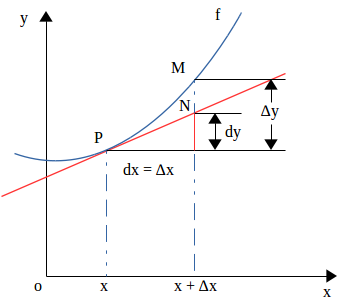
\includegraphics[scale=0.5]{./fig/derivative.png}
\caption{Derivative}
\label{fig:derivative}
\end{figure}

\begin{equation*}
f^{\prime}(x_0) = \lim_{\Delta x \to 0} \frac{\Delta y}{\Delta x} = \lim_{\Delta x \to 0} \frac{f(x_0 + \Delta x) - f(x_0)}{\Delta x}      
\end{equation*}

\textbf{Partial Derivative:}\\

\begin{equation*}
 \frac{\partial }{\partial x_j}f(x_0,x_1,\dots,x_n)= \lim_{\Delta x \to 0} \frac{\Delta y}{\Delta x} = \lim_{\Delta x \to 0} 
 \frac{f(x_0, \dots ,x_j + \Delta x,\dots,x_n) - f(x_0, \dots ,x_j,\dots,x_n)}{\Delta x}      
\end{equation*}

The derivative and the partial derivative are essentially same. Intuitively, the partial derivative is the rate of change of the function at a certain point along the positive direction of the coordinate axis. The partial derivative is the derivative with respect to one of the variables in a multivariate function.

\textbf{Directional Derivative:}\\

\begin{align*}
 \frac{\partial }{\partial l}f(x_0,x_1,\dots,x_n)&= \lim_{\rho \to 0} \frac{\Delta y}{\Delta x} \\
 &= \lim_{\rho \to 0} 
 \frac{f(x_0+\Delta x_0, \dots ,x_j + \Delta x_j,\dots,x_n+\Delta x_n) - f(x_0, \dots ,x_j,\dots,x_n)}{\rho}     \\
  \rho &= \sqrt{(\Delta x_0)^2 + \dots+(\Delta x_j)^2+\dots+(\Delta x_n)^2}
\end{align*}

In the definition of the preceding derivative and partial derivative, the change rate of the function is discussed along the positive direction of the coordinate axis. Then when we discuss the rate of change of the function in any direction, it also leads to the definition of the directional derivative, that is, the derivative value of a certain point in a direction of approach.

We must not only know the rate of change of the function in the positive direction of the coordinate axis (that is, the partial derivative), but also try to find the rate of change of the function in other specific directions. The directional derivative is the rate of change of the function in other specific directions.

\textbf{Gradient:}\\

\begin{equation*}
\mathbf{grad}f(x_0,x_1,\dots,x_n) = (\frac{\partial f}{\partial x_0},\dots,\frac{\partial f}{\partial x_j},\dots,\frac{\partial f}{\partial x_n})      
\end{equation*}

The gradient of a function at a point is such a vector whose direction is the same as the direction in which the maximum directional derivative, and its modulus is the maximum of the directional derivative.

\textbf{Gradient Descent:}\\

\begin{figure}[h]
\centering
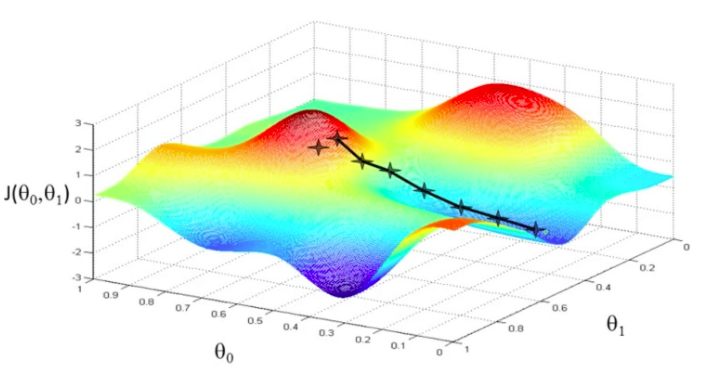
\includegraphics[scale=0.5]{./fig/gradient_descent.png}
\caption{Minimize cost function $J(\theta_0,\theta_1)$ with gradient descent}
\label{fig:gradient_descent}
\end{figure}

Since at some point in the variable space, the function has the greatest rate of change along the gradient direction, then when optimizing the objective function, it is natural to decrease the function value along the direction of the negative gradient to achieve our optimization goal.

\begin{equation*}
\mathbf{grad}f(x_0,x_1,\dots,x_n) = (\frac{\partial f}{\partial x_0},\dots,\frac{\partial f}{\partial x_j},\dots,\frac{\partial f}{\partial x_n})      
\end{equation*}

\begin{align*}
\textbf{repeat\{}\\
x_0 &:= x_0 - \alpha\frac{\partial f}{\partial x_0} \\
& \dots  \\
x_j &:= x_j - \alpha\frac{\partial f}{\partial x_j} \\
& \dots  \\
x_n &:= x_n - \alpha\frac{\partial f}{\partial x_n} \\
\}
\end{align*}

The condition for using the gradient descent method is that the direction of gradient points to the optimal solution direction, so the gradient direction is close to the optimal solution, and the gradient is very effective information about the optimal solution. On the simpler issues such as convex function and quasi convex function, it is indeed able to satisfy this condition, so the gradient descent can work well. However, when the optimization target has a large number of local extrema, most gradient directions of the solution space no longer point to the optimal solution, so in such cases the gradient method cannot get the optimal solution any more.

\section{Non-linear least squares}
The purpose of the \textbf{least squares} method is to find the least squares of error. There are two kinds of the \textbf{least squares} method: \textbf{linear} and \textbf{non-linear}. In this thesis we only consider the \textbf{non-linear} case. We usually use iterative methods(e.g. Gradient descent method; Gauss-Newton method) to solve \textbf{non-linear least squares} problem. We update the unknown variables to get closer to the approximation solution at each step with iterative method.

\begin{align*}
 \operatorname*{min}_x \norm{f(x)}^2_2  
\end{align*}

Now recall the camera model in previous section. Assume that we have \textit{n} object points in world coordinate, the \textit{i}-th point has it's corresponding projection on a plane with normalized image coordinate $x_i = [x_i,y_i]^T$. After adding the noise $\varepsilon_i$ on the error-free image coordinates $x_i$ we get noisy measurements of the image coordinates $ \tilde{x}= x_i + \varepsilon_i$. Thus, we can solve this reprojection error $\norm{\varepsilon_i}^2_2 = \norm{\tilde{x_i} - x_i}^2_2$ of each points with \textbf{least squares} method for the optimal pose $(\hat{R},\hat{t})$\cite{dynamic_markers}
%Dynamic Markers: Optimal control point configurations for homography and pose estimation
\begin{align*}
 (\hat{R},\hat{t}) = \operatorname*{argmin}_{R,t} \sum_{i=1}^{n}\norm{\varepsilon_i}^2_2  ,\qquad n \geq 3
\end{align*}


\begin{figure}[h]
\centering
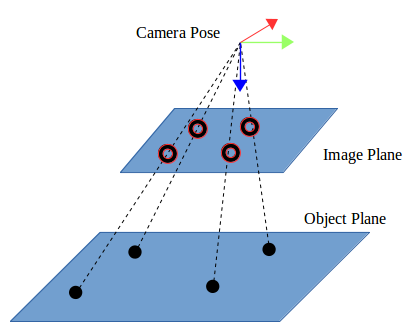
\includegraphics[scale=0.5]{./fig/least_squares.png}
\caption{Four Object points and their corresponding projection points in image plane with noisy, using least squares method to calculate the optimal camera post \textbf{R}, \textbf{t}}
\label{fig:least_squares}
\end{figure}